\documentclass[11pt,a4paper]{article}

% ----- PACKAGES -----
\usepackage[utf8]{inputenc}
\usepackage[T1]{fontenc}
\usepackage{helvet} % Modern sans-serif font
\renewcommand{\familydefault}{\sfdefault}
\usepackage{xcolor}
\usepackage{geometry}
\usepackage{tikz}
\usepackage{graphicx}
\usepackage{hyperref}
\usepackage{titlesec}
\usepackage{fancyhdr}
\usepackage{tcolorbox}
\usepackage{fontawesome5} % For icons
\usepackage{setspace}

% ----- GEOMETRY & LAYOUT -----
\geometry{
    top=3cm,
    bottom=3cm,
    left=2.5cm,
    right=2.5cm
}
\setstretch{1.2}

% ----- ORBYT BRAND COLORS -----
\definecolor{OrbytDark}{HTML}{0F172A}    % Slate 900 (Dark Background)
\definecolor{OrbytBlue}{HTML}{3B82F6}    % Blue 500 (Primary Accent)
\definecolor{OrbytLight}{HTML}{F8FAFC}   % Slate 50 (Light Background)
\definecolor{OrbytEmerald}{HTML}{10B981} % Emerald 500 (Success/Safety)
\definecolor{OrbytRed}{HTML}{EF4444}     % Red 500 (SOS/Alerts)
\definecolor{OrbytGray}{HTML}{64748B}    % Slate 500 (Muted Text)

% ----- HYPERREF SETUP -----
\hypersetup{
    colorlinks=true,
    linkcolor=OrbytBlue,
    filecolor=OrbytBlue,
    urlcolor=OrbytBlue,
}

% ----- CUSTOM SECTION FORMATTING -----
\titleformat{\section}
  {\normalfont\Large\bfseries\color{OrbytDark}}
  {\thesection}{1em}{}[\color{OrbytBlue}\titlerule]
\titleformat{\subsection}
  {\normalfont\large\bfseries\color{OrbytDark}}
  {\thesubsection}{1em}{}

% ----- HEADER & FOOTER -----
\pagestyle{fancy}
\fancyhf{}
\fancyhead[L]{\textbf{\textcolor{OrbytBlue}{ORBYT}} \textcolor{OrbytGray}{| The Intelligent Campus OS}}
\fancyfoot[C]{\thepage}
\renewcommand{\headrulewidth}{0.4pt}
\renewcommand{\headrule}{\hbox to\headwidth{\color{OrbytGray}\leaders\hrule height \headrulewidth\hfill}}

% ----- CUSTOM BOXES -----
\newtcolorbox{highlightbox}[1][]{
    colback=OrbytBlue!5!white,
    colframe=OrbytBlue,
    boxrule=1pt,
    arc=4pt,
    title=#1,
    coltitle=white,
    fonttitle=\bfseries
}

\newtcolorbox{alertbox}[1][]{
    colback=OrbytRed!5!white,
    colframe=OrbytRed,
    boxrule=1pt,
    arc=4pt,
    title=#1,
    coltitle=white,
    fonttitle=\bfseries
}

% ==========================================
% DOCUMENT BEGINS
% ==========================================
\begin{document}

% ----- TITLE PAGE -----
\begin{titlepage}
    \centering
    \vspace*{4cm}
    
    {\Huge \textbf{\textcolor{OrbytBlue}{ORBYT}}}\\[0.5cm]
    {\LARGE \textbf{\textcolor{OrbytDark}{The Intelligent Campus OS}}}\\[1.5cm]
    
    {\large \textbf{Project Documentation}}\\[0.5cm]
    {\large Problem Statement, Solution, and System Architecture}\\[2cm]
    
    
\begin{tikzpicture}
        % Decorative abstract Orbyt Logo / graphic
        \fill[OrbytBlue] (0,0) circle (1.5);
        \fill[OrbytDark] (0.8,0.8) circle (0.8);
        \fill[OrbytEmerald] (-0.8,-0.8) circle (0.5);
    \end{tikzpicture}\\[2cm]
    
    \vfill
    
    {\Large \textbf{Team: Black Squad}}\\[0.6cm]
    
    {\textbf{Prodhosh VS} \\ \texttt{prodhosh.vs2025@vitstudent.ac.in}}\\[0.4cm]
    {\textbf{Mohamed Nawaz N} \\ \texttt{mohamednawaz.n2025@vitstudent.ac.in}}\\[1.5cm]
    
    {\large Hackathon Submission}\\[0.2cm]
    {\textcolor{OrbytGray}{\today}}
    
\end{titlepage}

\newpage

% ----- TABLE OF CONTENTS -----
\tableofcontents
\newpage

% ----- SECTION 1: THE PROBLEM -----
\section{The Problem Statement}

Modern educational institutions suffer from extreme systemic fragmentation. Despite the rapid digitization of the world, universities and schools remain bogged down by legacy ERP systems that operate in isolated silos. Students, faculty, and administrators are forced to navigate dozens of disconnected portals, resulting in friction, inefficiency, and critical communication breakdowns.

\subsection{The Administrative \& Academic Disconnect}
\begin{itemize}
    \item \textbf{Data Silos:} A student's academic journey (attendance, grades, timetables) is entirely separated from their operational footprint (hostel room, transport routes, fee payments, library dues).
    \item \textbf{Cognitive Overload:} Students must remember multiple credentials and check multiple bulletin boards (both physical and digital) just to figure out where their next class is, whether a bus is delayed, or if a placement drive is happening.
    \item \textbf{The Extracurricular Chaos (The VIT Problem):} Discovering club recruitments, hackathons, and campus events relies entirely on fragmented, unorganized channels like scattered Instagram pages, endless WhatsApp groups, and word-of-mouth. This results in massive missed opportunities, spam, and a deeply messy student ecosystem.
    \item \textbf{Manual Bottlenecks:} Processes like hostel allocation, leave approvals, and grievance redressals often rely on paper trails or slow, unmonitored email chains, leading to weeks of delay and frustration.
\end{itemize}

\subsection{The Critical Crisis in Campus Safety}
Simultaneously, traditional ERP systems completely neglect \textbf{Campus Safety}. This is the most glaring vulnerability in modern institutions:
\begin{itemize}
    \item \textbf{No Immediate Recourse:} When emergencies occur—whether a medical crisis, harassment, or physical threat—students have no unified, instantaneous way to alert authorities. Calling a security guard's phone number is slow and unreliable.
    \item \textbf{Vulnerable Populations:} Women on campus, or students working late in labs, lack a discrete method (like a silent SOS) to share their live geolocation with campus security.
    \item \textbf{Blind Spots for Administration:} Campus administrators lack a real-time "Command Center" to view active incidents, track visitors entering the premises, or monitor transport fleets dynamically. 
\end{itemize}

The fundamental challenge is to create a platform that is not only unified and secure but also highly intelligent—capable of answering student queries intuitively, tracking live campus data, and providing a robust, instantaneous emergency response mechanism.

% ----- SECTION 2: THE SOLUTION (ORBYT) -----
\section{The Solution: ORBYT Campus OS}

\textbf{ORBYT} is an AI-powered, unified Campus Operating System that bridges the gap between academic administration, daily operations, and real-time campus safety. By acting as a single pane of glass, ORBYT eliminates silos and introduces a conversational, intelligent layer over all campus data.

\subsection{A Modular Yet Unified Ecosystem}
ORBYT provides specialized, role-based dashboards tailored exactly to what the user needs:
\begin{itemize}
    \item \textbf{For Students:} A central hub showing their live attendance threshold, their very next class (with room numbers), pending fee deadlines, and AI-curated placement opportunities based on their department.
    \item \textbf{Centralized Club Ecosystem:} A dedicated interface eliminating the "WhatsApp group chaos." Clubs can post active recruitments directly on the dashboard, allowing students to seamlessly discover, track, and apply to opportunities without relying on social media.
    \item \textbf{For Employees \& Faculty:} Streamlined tools to mark attendance, approve leave requests instantly, manage class schedules, and resolve student complaints without the paperwork.
    \item \textbf{For Administrators:} A bird's-eye "Command Center" providing real-time metrics on total campus headcount, active visitor logs, open infrastructure complaints, and crucially, live safety alerts.
\end{itemize}

\subsection{The "Zero-Latency" Safety Protocol}
Unlike traditional ERPs, ORBYT prioritizes human safety as a core feature, not an afterthought:
\begin{itemize}
    \item \textbf{One-Tap SOS:} A discrete, universally accessible SOS button instantly triggers a high-priority alert to the Admin Command Center, bypassing all standard notification routing.
    \item \textbf{Live Fleet Tracking:} Real-time simulated GPS tracking for campus transport ensures students (and parents) know exactly where their bus is, preventing students from waiting in unsafe, unlit areas.
    \item \textbf{Digital Visitor Management:} Strict, digital check-in/check-out logs for all campus visitors, accessible instantly by security personnel to prevent unauthorized access.
\end{itemize}

\subsection{AI as a First-Class Citizen}
ORBYT moves away from the "search and click" paradigm of legacy systems. Embedded directly into the platform is the \textbf{ORBYT AI Agent} (powered by Google Gemini), an omnipresent, intelligent campus companion.
\begin{itemize}
    \item \textbf{Conversational Data Access:} Instead of digging through menus, students can ask natural language questions: \textit{"What is my attendance?"}, \textit{"Which tech clubs are currently recruiting?"}, or \textit{"How do I report a broken AC in my hostel?"}
    \item \textbf{Context-Aware Intelligence:} The AI agent is deeply integrated with the campus database. It instantly retrieves personalized answers, significantly reducing the administrative burden on faculty and staff who typically answer these redundant queries.
\end{itemize}

\begin{alertbox}[Design Philosophy]
ORBYT is designed to reduce cognitive load. Utilizing a premium, modern UI with dynamic Dark Mode, the interface minimizes distractions so critical information—like an active safety alert or a low attendance warning—stands out immediately.
\end{alertbox}

% ----- SECTION 3: ARCHITECTURE -----
\section{System Architecture}

ORBYT is engineered for speed, scale, and absolute cross-platform reliability. It utilizes a modern, decoupled serverless architecture designed to handle thousands of concurrent users with minimal latency.

\subsection{Frontend Architecture: Next.js 14 \& React Server Components}
The client interface is built using the \textbf{Next.js App Router} paradigm. By strategically combining React Server Components (RSC) and Client Components, ORBYT drastically reduces the JavaScript bundle size shipped to the browser. 
\begin{itemize}
    \item \textbf{Layout Nesting:} The application utilizes deeply nested layouts (e.g., \texttt{app/dashboard/layout.tsx}) to preserve state (like the Sidebar and Theme Providers) across navigations without re-rendering the entire DOM.
    \item \textbf{Headless UI Primitives:} To ensure absolute accessibility and keyboard navigation, ORBYT uses headless primitives (Radix UI / Base UI) styled exclusively with \textbf{Tailwind CSS v4}, ensuring zero-runtime CSS generation and a highly premium aesthetic.
\end{itemize}

\subsection{Database \& Authentication: Supabase Ecosystem}
ORBYT relies on Supabase as its robust backend-as-a-service, sitting on top of a highly relational PostgreSQL database.
\begin{itemize}
    \item \textbf{Strict Identity Verification:} Authentication is handled via secure JWTs. Upon login, users are mapped from the \texttt{auth.users} schema to the \texttt{public.profiles} table via strict Foreign Key constraints, ensuring absolute data integrity.
    \item \textbf{Row Level Security (RLS):} The cornerstone of ORBYT's security is PostgreSQL RLS. Policies dictate that a student can \textit{only} query their own attendance and fees at the database level, preventing any horizontal privilege escalation, while Admin tokens possess global \texttt{SELECT} privileges.
\end{itemize}

\subsection{AI Streaming Pipeline: Google Gemini 2.5}
To provide a zero-latency conversational experience, ORBYT integrates Google Gemini via an Edge-compatible API route (\texttt{/api/chat/route.ts}).
\begin{itemize}
    \item \textbf{Contextual Injection:} The user's query is appended to a massive, dynamically generated system prompt containing relevant campus knowledge, essentially functioning as a highly optimized Retrieval-Augmented Generation (RAG) pipeline.
    \item \textbf{Chunked Streaming (SSE):} Instead of forcing the user to wait for the entire AI response to generate, the backend utilizes \texttt{generateContentStream}. It encodes the response via \texttt{TextEncoder} and sends it to the client using Server-Sent Events (SSE) and a \texttt{ReadableStream}, allowing the UI to type out the response in real-time.
\end{itemize}

\subsection{Data Flow \& Security Diagram}

\begin{center}
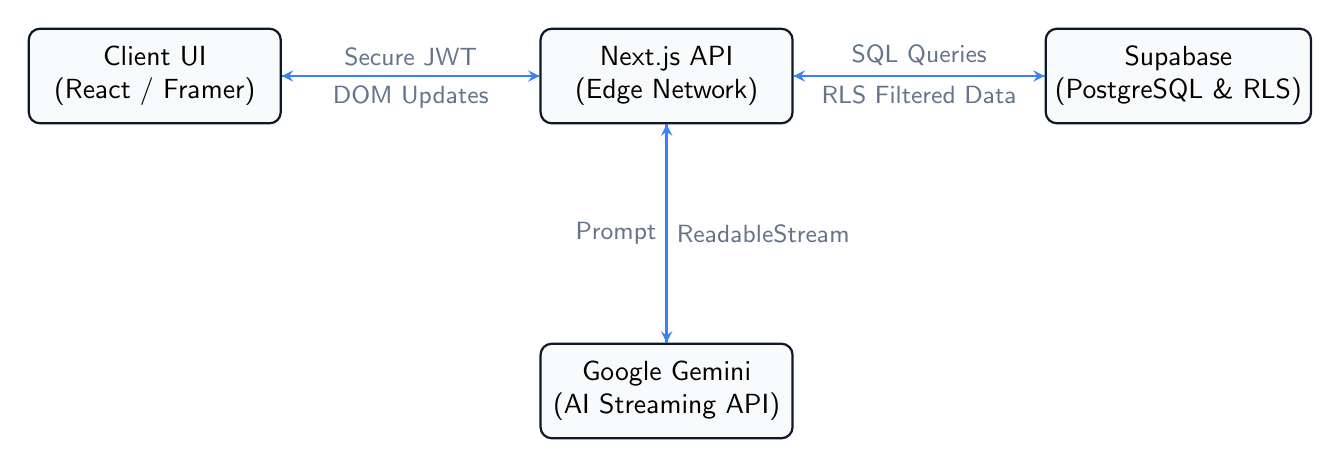
\begin{tikzpicture}[
    node distance=2.5cm,
    box/.style={rectangle, draw=OrbytDark, rounded corners, fill=OrbytLight, thick, minimum width=3.2cm, minimum height=1.2cm, align=center},
    arrow/.style={->, thick, OrbytBlue, >=stealth}
]

% Nodes
\node[box] (client) {Client UI \\ (React / Framer)};
\node[box, right of=client, xshift=4cm] (api) {Next.js API \\ (Edge Network)};
\node[box, right of=api, xshift=4cm] (db) {Supabase \\ (PostgreSQL \& RLS)};
\node[box, below of=api, yshift=-1.5cm] (ai) {Google Gemini \\ (AI Streaming API)};

% Arrows
\draw[arrow] (client) -- node[above, text=OrbytGray, font=\small] {Secure JWT} (api);
\draw[arrow] (api) -- node[below, text=OrbytGray, font=\small] {DOM Updates} (client);

\draw[arrow] (api) -- node[above, text=OrbytGray, font=\small] {SQL Queries} (db);
\draw[arrow] (db) -- node[below, text=OrbytGray, font=\small] {RLS Filtered Data} (api);

\draw[arrow] (api) -- node[left, text=OrbytGray, font=\small] {Prompt} (ai);
\draw[arrow] (ai) -- node[right, text=OrbytGray, font=\small] {ReadableStream} (api);

\end{tikzpicture}
\end{center}

\end{document}
